\documentclass[12pt,a4paper]{article}

% --- Packages ---
\usepackage[utf8]{inputenc}
\usepackage[english]{babel}
\usepackage[margin=2.5cm]{geometry}
\usepackage{setspace}
\onehalfspacing
% Formatting & Table Packages
\usepackage{array}
\usepackage{tabularx}
\usepackage{booktabs}
\usepackage{multirow}
\usepackage{colortbl}
\usepackage{xcolor}
\usepackage{enumitem}
\usepackage{caption}
\usepackage{longtable}
\usepackage{graphicx}
\graphicspath{{images/}}
\usepackage{microtype}
\usepackage{indentfirst}

\setlength{\parindent}{0pt}
\setlength{\parskip}{0pt}

% Header & Footer
\usepackage{fancyhdr}
\pagestyle{fancy}
\fancyhf{}
\renewcommand{\headrulewidth}{0pt}
\renewcommand{\footrulewidth}{0pt}
\cfoot{\thepage}

% Hyperlinks & PDF Metadata
\usepackage{hyperref}

\hypersetup{
    colorlinks=true,
    linkcolor=black,
    citecolor=black,
    urlcolor=blue!80!black,
    pdftitle={Software Requirements Specification - AI-powered Film Photography Contest Management Platform},
    pdfauthor={Group 7}
}

% Colors
\definecolor{headerblue}{RGB}{220,235,252}
\definecolor{altrowgray}{RGB}{248,249,250}

\begin{document}

\begin{titlepage}
    \thispagestyle{empty}

    \begin{center}

        % University
        {\large\bfseries UNIVERSITY OF TRANSPORT HO CHI MINH CITY}\\[0.15cm]
        {\normalsize\bfseries FACULTY OF INFORMATION TECHNOLOGY}\\[0.15cm]

        \rule{0.35\textwidth}{0.5pt}

        % Move the title and table downward
        \vfill

        % Project title
        {\Huge\bfseries Capstone Project Document}\\[0.3cm]
        \rule{0.5\textwidth}{0.5pt}\\[1.5cm]

        % Project information table
        \renewcommand{\arraystretch}{1.1}

        \makebox[\textwidth][c]{%
        \begin{tabularx}{0.90\textwidth}{|
            >{\centering\arraybackslash}p{4.2cm}|
            >{\centering\arraybackslash}X|}
            
            \hline

            % Project name - full width
            \multicolumn{2}{|c|}{%
                \begin{minipage}{0.85\textwidth}
                    \centering
                    \vspace{0.2cm}
                    \textbf{\large AI-powered Film Photography Contest Management Platform}
                    \vspace{0.2cm}
                \end{minipage}
            }
            \\[0.5em]
            \hline

            \bfseries Group Members:
            & Tran Phat Tai - 086206011804\\
            & Tran Quy Minh Thien - 079207025398\\
            & Vo Quoc Khanh - 066207017208\\
            & Nguyen Thi My Uyen - 068307002174\\
            & Huynh Nguyen Duy Tan - 054207001780\\
            \hline

            \bfseries Lecturer:
            & Nguyen Van Chien\\
            \hline

        \end{tabularx}
        }

        \vfill

        % Date
        {\small - Ho Chi Minh City, September 2026 -}

    \end{center}
\end{titlepage}

\newpage

\pagenumbering{arabic}
\setcounter{page}{2}

\pdfbookmark[1]{Contents}{toc}
\begingroup
\setcounter{tocdepth}{4}
\renewcommand{\contentsname}{\centering Contents}
\tableofcontents
\endgroup
\newpage

\begingroup
\setlength{\parindent}{1.5em}
\setlength{\parskip}{0.8em}
\section*{Acknowledgement}
\addcontentsline{toc}{section}{Acknowledgement}

The completion of this Software Requirements Specification (SRS) and the AI-powered Film Photography Contest Management Platform project would not have been possible without the support and guidance of many individuals.

First and foremost, we would like to express our deepest gratitude to the lecturers and the board of University of Transport Ho Chi Minh City. The dynamic learning environment and practical curriculum at University of Transport Ho Chi Minh City have provided us with a solid foundation in Software Engineering and Business Analysis, enabling us to approach this project with confidence.

We are especially grateful to our supervisor. Your dedicated guidance, valuable insights, and constructive criticism throughout the semester have been instrumental in shaping this project. Your expertise helped us navigate complex challenges, from defining use cases and screen flows to finalizing this SRS document according to industry standards.

Finally, although we have worked hard to ensure accuracy, errors may still exist. We welcome any feedback and suggestions from our lecturers to further improve this project.
\endgroup

\section*{Definition and Acronyms}
\addcontentsline{toc}{section}{Definition and Acronyms}

\begin{longtable}{|p{2.2cm}|p{4.4cm}|p{7.0cm}|}
    \hline
    \rowcolor{headerblue} \textbf{Acronym} & \textbf{Definition} & \textbf{Description} \\ \hline
    \endfirsthead
    \hline
    \rowcolor{headerblue} \textbf{Acronym} & \textbf{Definition} & \textbf{Description} \\ \hline
    \endhead
    \endfoot
    \endlastfoot
    \textbf{API} & Application Programming Interface & A set of rules and protocols that allows different software applications to communicate with each other. \\ \hline
    \textbf{BA} & Business Analysis & The practice of enabling change in an enterprise by defining needs and recommending solutions that deliver value to stakeholders. \\ \hline
    \textbf{BR} & Business Rule & A rule that defines or constrains some aspect of business and always resolves to either true or false. \\ \hline
    \textbf{ERD} & Entity Relationship Diagram & A flowchart that illustrates how "entities" such as people, objects, or concepts relate to each other within a system. \\ \hline
    \textbf{EXIF} & Exchangeable Image File Format & A standard format for specifying metadata tags embedded in digital image files (e.g., Camera Model, Lens, Film Stock/ISO). \\ \hline
    \textbf{GUI} & Graphical User Interface & A type of user interface that allows users to interact with electronic devices through graphical icons and visual indicators. \\ \hline
    \textbf{MHs} & Man-Hours & An estimated unit of work equal to one hour of continuous labor by one project team member. \\ \hline
    \textbf{pHash} & Perceptual Hashing & A fingerprinting algorithm used to analyze image contents and generate a unique hash for duplicate image detection. \\ \hline
    \textbf{PM} & Project Manager & The person responsible for planning, executing, monitoring, controlling, and closing projects. \\ \hline
    \textbf{RBAC} & Role-Based Access Control & A security approach that restricts system access based on defined user roles (e.g., Candidate, Judge, Organizer). \\ \hline
    \textbf{SDD} & Software Design Description & A document that describes the design of a software system, including its architecture, components, and interfaces. \\ \hline
    \textbf{SPMP} & Software Project Management Plan & A document that defines the project plan, specifying the tasks, schedule, resources, and management approach. \\ \hline
    \textbf{SRS} & Software Requirement Specification & A document that describes what the software will do and how it will be expected to perform. \\ \hline
    \textbf{UAT} & User Acceptance Test & The final phase of the software testing process where actual software users test the software to make sure it can handle required tasks in real-world scenarios. \\ \hline
    \textbf{UC} & Use Case & A list of actions or event steps typically defining the interactions between a role and a system to achieve a goal. \\ \hline
\end{longtable}

\newpage

\section{Project Introduction}
\label{sec:project_introduction}

\subsection{Overview}
\label{subsec:overview}

\subsubsection{Project Information}
\label{subsubsec:project_info}

\textbf{Project Name:} AI-powered Film Photography Contest Management Platform\\
\textbf{Software Type:} Web Application\\
\textbf{Purpose:} To streamline the organization, submission, judging, and exhibition processes of film photography competitions.\\
\textbf{Group Name:} Group 7

\subsection{Project Team}
\label{subsec:project_team}

\begin{tabularx}{\textwidth}{|l|l|X|}
    \hline
    \textbf{Full Name} & \textbf{Role} & \textbf{Email} \\
    \hline
    Nguyen Van Chien & Lecturer & \href{mailto:chiennv@ut.edu.vn}{chiennv@ut.edu.vn} \\
    \hline
    Tran Phat Tai & Leader & \href{mailto:taitp1804@ut.edu.vn}{taitp1804@ut.edu.vn} \\
    \hline
    Tran Quy Minh Thien & Member & \href{mailto:thientqm795398@ut.edu.vn}{thientqm795398@ut.edu.vn} \\
    \hline
    Vo Quoc Khanh & Member & \href{mailto:khanhvq667208@ut.edu.vn}{khanhvq667208@ut.edu.vn} \\
    \hline
    Nguyen Thi My Uyen & Member & \href{mailto:uyenntm682174@ut.edu.vn}{uyenntm682174@ut.edu.vn} \\
    \hline
    Huynh Nguyen Duy Tan & Member & \href{mailto:tanhnd541780@ut.edu.vn}{tanhnd541780@ut.edu.vn} \\
    \hline
\end{tabularx}

% ----------------------------------------------------
\subsection{Product Background}
\label{subsec:product_background}
\begingroup
\setlength{\parindent}{1.5em}
\setlength{\parskip}{0.8em}

Film photography has become increasingly popular in recent years, leading to a growing number of photography contests. However, most contests are still managed using separate tools such as online forms, spreadsheets, emails, and cloud storage, resulting in inefficient workflows and difficulties in submission verification, judging, and data management.

Unlike digital photography contests, film photography requires additional technical metadata such as film stock, camera, lens, ISO, developing laboratory, and scanning information. Existing contest management systems generally do not support these specialized requirements.

To address these limitations, this project proposes an AI-powered Film Photography Contest Management Platform. The platform centralizes contest management, supports film-specific metadata, and integrates AI for duplicate image detection, AI-generated image detection, automatic image categorization, and contest analytics, improving efficiency, transparency, and fairness throughout the competition process.
\endgroup

% ----------------------------------------------------
\subsection{Existing Systems}
\label{subsec:existing_systems}

\subsubsection{Picter}
\label{subsubsec:picter}

\textbf{Link:} \url{https://www.picter.com}\\
\textbf{Description:} A professional platform for managing photography competitions, open calls, grants, and awards. It is widely used by organizations such as World Press Photo, Leica, and Magnum.\\
\textbf{Actors:} Organizers, judges, photographers, administrators.\\
\textbf{Key Features:}
\begin{itemize}
    \item Online contest creation and management.
    \item Photo submission and portfolio management.
    \item Online judging and scoring.
    \item Result publication and digital archive.
\end{itemize}
\textbf{Pros:} Complete end-to-end contest management; professional judging workflow; supports large-scale international competitions.\\
\textbf{Cons:} Not designed specifically for film photography; does not provide film-specific metadata management (film stock, camera, developing lab, etc.); limited AI verification features.

\subsubsection{CameraComp}
\label{subsubsec:cameracomp}

\textbf{Link:} \url{https://www.cameracomp.com}\\
\textbf{Description:} A cloud-based competition management system developed for photography clubs and federations.\\
\textbf{Actors:} Club administrators, judges, photographers.\\
\textbf{Key Features:}
\begin{itemize}
    \item Competition management.
    \item Image submission.
    \item Online and offline judging.
    \item Member and event management.
\end{itemize}
\textbf{Pros:} Simple and intuitive interface; integrated competition and member management; supports multiple judging methods.\\
\textbf{Cons:} Focuses on photography clubs rather than film photography contests; no AI-generated image detection; no film metadata management.

Compared with the systems above, the proposed platform is specifically designed for film photography contests. It focuses on film-specific metadata, AI-based verification, and a more specialized workflow for organizers, judges, and participants.

% ----------------------------------------------------
\subsection{Business Opportunity}
\label{subsec:business_opportunity}
\begingroup
\setlength{\parindent}{1.5em}
\setlength{\parskip}{0.8em}

The growing popularity of film photography has increased the demand for efficient contest management. However, most organizers still use separate tools, making submission management, judging, and verification inefficient. This project provides a centralized platform with AI support to improve efficiency, transparency, and fairness for photography contests.
\endgroup

% ----------------------------------------------------
\subsection{Software Product Vision}
\label{subsec:software_product_vision}
\begingroup
\setlength{\parindent}{1.5em}
\setlength{\parskip}{0.8em}

The project aims to develop a web and mobile platform for managing film photography contests. It supports the complete contest workflow, from registration and submission to judging and result publication, while integrating AI for duplicate image detection, AI-generated image detection, and automated image categorization to enhance contest management.
\endgroup

% ----------------------------------------------------
\subsection{Project Scope \& Limitations}
\label{subsec:project_scope_limitations}

\subsubsection{Major Features}
\label{subsubsec:major_features}

The following primary functional modules are included:

\begin{itemize}[leftmargin=*, itemsep=0.3em]
    \item \textbf{FE1 – User \& Role Management:} Provides authentication, role-based access control (RBAC), and profile management for Candidates, Judges, and Organizers/Admins.
    \item \textbf{FE2 – Contest Management:} Enables Organizers to create and configure new contests, set submission rules, manage timelines, oversee participant lists, and assign judges.
    \item \textbf{FE3 – Submission System:} Allows candidates to upload high-resolution film scan images, input detailed technical specifications (EXIF metadata, Camera, Lens, Film Stock/ISO, Aperture, Shutter Speed), and track submission statuses.
    \item \textbf{FE4 – Judging \& Evaluation:} Provides a dedicated judging panel featuring high-resolution image viewing tools (Zoom/Pan), multi-criteria evaluation scoring, and feedback/commenting capabilities.
    \item \textbf{FE5 – Automated Processing \& Anti-cheat:} Automatically extracts EXIF data from uploaded images and utilizes perceptual hashing (pHash) with Hamming distance calculations to detect and flag potential image plagiarism or duplicate submissions.
    \item \textbf{FE6 – Exhibition Gallery:} A public online gallery showcasing winning or selected submissions, equipped with advanced filtering options by Film Stock, Camera model, or Contest.
\end{itemize}

\subsubsection{Limitations \& Exclusions}
\label{subsubsec:limitations_exclusions}

The following points detail the operational constraints and out-of-scope boundaries:

\begin{itemize}[leftmargin=*, itemsep=0.3em]
    \item \textbf{LI-01:} File size and format restrictions: Supports only \texttt{.jpg}, \texttt{.jpeg}, and \texttt{.png} formats, with file sizes strictly limited between 2 MB and 25 MB.
    \item \textbf{LI-02:} Automated metadata extraction depends entirely on intact EXIF data within uploaded film scan files; stripped EXIF files require manual input and administrative flagging.
    \item \textbf{LI-03:} Perceptual hashing (pHash) and Hamming distance duplication detection are processed asynchronously via message queues, resulting in slight processing delays rather than real-time feedback upon upload.
    \item \textbf{LI-04:} No support for native mobile applications (iOS/Android); the system is strictly developed as a responsive web application.
    \item \textbf{LI-05:} No integration with online payment gateways or photo editing/post-processing tools (candidates must upload finalized image files, and all financial transactions are out of scope).
\end{itemize}

% --- Chapter II: Project Management Plan ---
\newpage

\section*{II. Project Management Plan}
\addcontentsline{toc}{section}{II. Project Management Plan}
\setcounter{section}{2}

% Number subsections in this chapter as 2, 3, ... (Chapter I style)
\renewcommand{\thesubsection}{\arabic{subsection}}
\setcounter{subsection}{0}

\subsection{Overview}

\subsubsection{Scope \& Estimation}
\label{subsubsec:ii_scope}

% Breakable table using longtable; column widths as fractions of \textwidth for balanced layout
\begin{longtable}{|>{\centering\arraybackslash}p{0.06\textwidth}|>{\raggedright\arraybackslash}p{0.62\textwidth}|>{\centering\arraybackslash}p{0.12\textwidth}|>{\centering\arraybackslash}p{0.16\textwidth}|}
\hline
\multicolumn{1}{|c|}{\textbf{WBS}} & \multicolumn{1}{c|}{\textbf{Item}} & \multicolumn{1}{c|}{\textbf{Complexity}} & \multicolumn{1}{c|}{\begin{tabular}[c]{@{}c@{}}\textbf{Est. Effort}\\\textbf{(MHs)}\end{tabular}} \\
\hline
\endfirsthead
\multicolumn{1}{|c|}{\textbf{WBS}} & \multicolumn{1}{c|}{\textbf{Item}} & \multicolumn{1}{c|}{\textbf{Complexity}} & \multicolumn{1}{c|}{\begin{tabular}[c]{@{}c@{}}\textbf{Est. Effort}\\\textbf{(MHs)}\end{tabular}} \\
\hline
\endhead
\hline
\endfoot
\hline
\endlastfoot

1 & \textbf{FE01. User \& Role Management} & & 40 \\
\hline
1.1 & Authentication System (Login, Register, OAuth Google, JWT) & Simple & 10 \\
\hline
1.2 & Password Recovery \& Email Verification & Simple & 8 \\
\hline
1.3 & User Profile \& Portfolio Management & Medium & 10 \\
\hline
1.4 & Role-Based Access Control (RBAC) \& User Management (Admin) & Medium & 12 \\
\hline

2 & \textbf{FE02. Contest Management} & & 48 \\
\hline
2.1 & Contest Creation \& Basic Setup (Rules, Prizes, Categories) & Medium & 14 \\
\hline
2.2 & Timeline \& Phase Transition Configuration (Auto Scheduler) & Medium & 12 \\
\hline
2.3 & Jury Assignment \& Judging Criteria Setup & Medium & 12 \\
\hline
2.4 & Contest Status Management \& Moderator Dashboard & Simple & 10 \\
\hline

3 & \textbf{FE03. Submission System} & & 64 \\
\hline
3.1 & Presigned Cloud Storage Upload (S3/Cloudinary) for Hi-Res Scan & Complex & 20 \\
\hline
3.2 & Film Specifications \& Metadata Input Form (Film Stock, Camera, Lens) & Medium & 14 \\
\hline
3.3 & Negative Film / Contact Sheet Proof Attachment Upload & Medium & 16 \\
\hline
3.4 & Submission Drafts \& Candidate Entry History & Simple & 14 \\
\hline

4 & \textbf{FE04. Judging \& Evaluation} & & 56 \\
\hline
4.1 & Blind Judging Portal (Anonymized Candidate Data) & Medium & 12 \\
\hline
4.2 & High-Resolution Image Viewer (Zoom/Pan HD \& Negative Inspector) & Medium & 16 \\
\hline
4.3 & Multi-Criteria Scoring System \& Feedback Panel & Complex & 16 \\
\hline
4.4 & Final Leaderboard Calculation \& Winner Approval & Medium & 12 \\
\hline

5 & \textbf{FE05. Automated Processing \& Anti-cheat (AI Subsystem)} & & 72 \\
\hline
5.1 & Auto EXIF Metadata Extraction Engine & Medium & 18 \\
\hline
5.2 & EXIF vs User Declaration Mismatch Verification & Medium & 14 \\
\hline
5.3 & pHash Duplication Detection \& Fingerprinting Algorithm & Complex & 24 \\
\hline
5.4 & Fraud Flagging System \& Admin Inspection Dashboard & Medium & 16 \\
\hline

6 & \textbf{FE06. Exhibition Gallery \& Community} & & 32 \\
\hline
6.1 & Public Gallery \& Masonry Display Grid & Simple & 8 \\
\hline
6.2 & Advanced Filtering (Film Stock, Camera Model, Contest, Year) & Medium & 10 \\
\hline
6.3 & Public Voting \& Anti-Spam Community Engagement & Medium & 8 \\
\hline
6.4 & Social Sharing \& Certificate Generation for Winners & Simple & 6 \\
\hline

7 & \textbf{FE07. System Architecture, QA \& DevOps} & & 88 \\
\hline
7.1 & SRS / SDD Documentation \& System Architecture Design & Medium & 24 \\
\hline
7.2 & Database Schema Design (ERD) \& Base API Setup & Medium & 16 \\
\hline
7.3 & QA Test Plan, Test Cases Execution \& Bug Fixing & Medium & 30 \\
\hline
7.4 & Docker Containerization, CI/CD Pipeline \& Deployment & Medium & 18 \\
\hline

\multicolumn{3}{|r|}{\textbf{TOTAL}} & \textbf{400 MHs} \\
\hline

\end{longtable}

\subsubsection{Project Objectives}
\label{subsubsec:ii_objectives}

\begin{table}[ht]
\centering
\small
\renewcommand{\arraystretch}{1.05}
\setlength{\tabcolsep}{4pt}
\begin{tabularx}{\textwidth}{|>{\raggedright\arraybackslash}p{0.16\textwidth}|>{\raggedright\arraybackslash}X|>{\raggedright\arraybackslash}p{0.14\textwidth}|>{\centering\arraybackslash}p{0.12\textwidth}|>{\raggedright\arraybackslash}X|}
\hline
\multicolumn{1}{|c|}{\begin{tabular}[c]{@{}c@{}}\textbf{Testing}\\\textbf{Stage}\end{tabular}} & \multicolumn{1}{c|}{\begin{tabular}[c]{@{}c@{}}\textbf{Test}\\\textbf{Coverage}\end{tabular}} & \multicolumn{1}{c|}{\begin{tabular}[c]{@{}c@{}}\textbf{No. of}\\\textbf{Defects}\end{tabular}} & \multicolumn{1}{c|}{\begin{tabular}[c]{@{}c@{}}\textbf{\% of}\\\textbf{Defect}\end{tabular}} & \multicolumn{1}{c|}{\textbf{Notes}} \\
\hline
Reviewing & 100\% artifacts reviewed (SRS, SDD, ERD, Wireframes) & - & - & Peer review and supervisor feedback \\
\hline
Unit Test & $\geq$ 70\% code coverage for Core BE and AI modules & 0 critical; $\leq$ 10 minor & $\leq$ 10\% & Automated testing (JUnit, Jest, PyTest for AI functions) \\
\hline
Integration Test & $\geq$ 85\% API and async pipeline coverage & 0 critical; $\leq$ 8 minor & $\leq$ 8\% & Postman / Swagger and S3 upload / AI queue testing \\
\hline
System Test & $\geq$ 95\% major features (Contest, Submission, AI Inspection, Judging) & 0 critical; $\leq$ 5 minor & $\leq$ 5\% & Staging environment regression and performance testing for high-resolution uploads \\
\hline
Acceptance Test (UAT) & 100\% critical user flows and AI verification accuracy & 0 critical / blocker & 0\% & UAT with stakeholders (organizers, jury, candidates) \\
\hline
\end{tabularx}
\end{table}

\subsubsection{Project Risks}
\label{subsubsec:ii_risks}

\begin{center}
\small
\renewcommand{\arraystretch}{1.08}
\setlength{\tabcolsep}{4pt}
\begin{tabularx}{\textwidth}{|>{\centering\arraybackslash}p{0.06\textwidth}|>{\raggedright\arraybackslash}X|>{\centering\arraybackslash}p{0.12\textwidth}|>{\centering\arraybackslash}p{0.14\textwidth}|>{\raggedright\arraybackslash}X|}
\hline
\multicolumn{1}{|c|}{\textbf{No.}} & \multicolumn{1}{c|}{\begin{tabular}[c]{@{}c@{}}\textbf{Risk}\\\textbf{Description}\end{tabular}} & \multicolumn{1}{c|}{\textbf{Impact}} & \multicolumn{1}{c|}{\textbf{Possibility}} & \multicolumn{1}{c|}{\begin{tabular}[c]{@{}c@{}}\textbf{Response}\\\textbf{Plans}\end{tabular}} \\
\hline
1 & Changing requirements from stakeholders (organizers, jury) & Medium & Medium & Baseline SRS plus change control process; weekly review and sign-off with supervisor \\
\hline
2 & Limited domain knowledge in film photography (film stocks, EXIF structures, scan types) and AI anti-cheat models & High & Medium & Consult film photography experts/advisors; early PoC for EXIF extraction and pHash algorithm; prototype feedback \\
\hline
3 & Third-party integrations and services (AWS S3 / Cloudinary for high-resolution image storage, Docker, Redis, Resend / SMTP) are unstable or exceed free-tier limits & Medium & Medium & Early PoC in sandbox; image compression and thumbnail generation; retries and fallback mechanisms; service cost monitoring \\
\hline
4 & Data privacy and security (protecting unpublished contest entries and candidate PII) & High & Low & Implement RBAC, anonymized submission pipeline for blind judging, S3 presigned URLs with expiration, and data encryption at rest and in transit \\
\hline
5 & Resource availability or absence among team members & Medium & Medium & Cross-training tech stacks (front-end / back-end / AI); backup feature ownership; daily standups; sprint buffer time \\
\hline
6 & Performance degradation under peak loads (simultaneous high-resolution image uploads near contest deadline) & High & Medium & Direct-to-S3 presigned upload (bypass core server); Redis caching; asynchronous background AI processing queue; rate limiting and load testing in Sprint 6 \\
\hline
\end{tabularx}
\end{center}

\subsection{Management Approach}
\label{subsec:ii_management_approach}

\subsubsection{Project Process}
\label{subsubsec:ii_project_process}

\textbf{Methodology:} The project applies the Agile Scrum methodology.\\
\textbf{Iteration Model:} 1-week sprints, total of 7 sprints (7 weeks).\\
\textbf{Sprint Breakdown:}
\begin{itemize}[leftmargin=*, itemsep=0.3em]
    \item \textbf{Sprint 1:} Project initiation, requirement elicitation (SRS), architecture \& DB design (SDD), UI/UX wireframing, and AI Proof of Concept (EXIF \& pHash).
    \item \textbf{Sprint 2:} Development of FE01 (User Authentication, Profile Management, \& RBAC).
    \item \textbf{Sprint 3:} Development of FE02 (Contest Creation, Timeline, \& Jury Assignment).
    \item \textbf{Sprint 4:} Development of FE03 (Submission System with Presigned S3 Upload \& Film Specifications).
    \item \textbf{Sprint 5:} Development of FE04 (Blind Judging Portal, HD Image Viewer, \& Scoring System).
    \item \textbf{Sprint 6:} Development of FE05 (AI Processing Pipeline: Auto EXIF \& pHash Duplicate Detection) \& FE06 (Exhibition Gallery).
    \item \textbf{Sprint 7:} FE07 Integration, System Testing, Bug Fixing, UAT, Docker Containerization, \& Cloud Deployment.
\end{itemize}
\textbf{Scrum Ceremonies:} Daily Stand-up (15 minutes), Weekly Sprint Planning, Sprint Review, and Sprint Retrospective.\\
\textbf{Artifacts:} Product Backlog, Sprint Backlog, Burndown Chart, Weekly Working Increment.

\subsubsection{Quality Management}
\label{subsubsec:ii_quality_management}

The quality objective is to ensure a stable, accurate, secure, and performant platform for managing film photography contests and automated image inspection within the 7-week timeframe.\\
The approach includes:
\begin{itemize}[leftmargin=*, itemsep=0.5em]
    \item \textbf{Defect Prevention:}
    \begin{itemize}[label={-}, leftmargin=1.5em, itemsep=0.2em]
        \item Enforce clean code conventions and modular architecture (Separation of Core API and AI Services).
        \item Database normalization (PostgreSQL), constraints, and indexing for fast query performance on media records.
    \end{itemize}
    \item \textbf{Reviewing:}
    \begin{itemize}[label={-}, leftmargin=1.5em, itemsep=0.2em]
        \item Mandatory Code Review with at least 1 Peer Reviewer and Leader approval before merging Pull Requests.
        \item Peer review for technical documentation (SRS, SDD, ERD, Test Cases).
    \end{itemize}
    \item \textbf{Unit Testing:}
    \begin{itemize}[label={-}, leftmargin=1.5em, itemsep=0.2em]
        \item \textbf{Tools:} Jest/React Testing Library (Frontend), JUnit/PyTest (Core BE \& AI Engine).
        \item \textbf{Goal:} $\geq$ 70\% code coverage, focusing on critical API logic, EXIF parsers, and hashing algorithm utilities.
    \end{itemize}
    \item \textbf{Integration Testing:}
    \begin{itemize}[label={-}, leftmargin=1.5em, itemsep=0.2em]
        \item \textbf{Tools:} Postman / Newman for REST API workflows.
        \item \textbf{Scope:} Asynchronous task queue handling (Redis/Celery) for background image processing and Direct-to-Cloud (AWS S3 / Cloudinary) presigned upload pipelines.
    \end{itemize}
    \item \textbf{System Testing:}
    \begin{itemize}[label={-}, leftmargin=1.5em, itemsep=0.2em]
        \item Conducted in Week 7 on a Staging Environment hosted on AWS / Cloud VPS.
        \item Full regression testing of all modules (FE01 to FE07).
        \item Performance and Load Testing (using Apache JMeter or K6) for peak submission scenarios near contest deadlines and Hi-Res image viewing.
    \end{itemize}
    \item \textbf{Acceptance Testing (UAT):}
    \begin{itemize}[label={-}, leftmargin=1.5em, itemsep=0.2em]
        \item User Acceptance Testing (Week 7) with primary stakeholders: Contest Organizers, Jury Members, and Candidates/Photographers.
        \item Ensure 100\% of critical flows (Contest creation, Entry submission, AI flagging, and Blind judging) pass successfully before final presentation.
    \end{itemize}
\end{itemize}

\subsubsection{Training Plan}
\label{subsubsec:ii_training_plan}

\renewcommand{\arraystretch}{1.1}
\setlength{\tabcolsep}{6pt}
\begin{longtable}{|>{\raggedright\arraybackslash}p{0.30\textwidth}|>{\raggedright\arraybackslash}p{0.20\textwidth}|>{\raggedright\arraybackslash}p{0.16\textwidth}|>{\raggedright\arraybackslash}p{0.28\textwidth}|}
\hline
\multicolumn{1}{|c|}{\textbf{Training Area}} & \multicolumn{1}{c|}{\textbf{Participants}} & \multicolumn{1}{c|}{\begin{tabular}[c]{@{}c@{}}\textbf{When,}\\\textbf{Duration}\end{tabular}} & \multicolumn{1}{c|}{\begin{tabular}[c]{@{}c@{}}\textbf{Waiver}\\\textbf{Criteria}\end{tabular}} \\
\hline
Next.js / ReactJS (Frontend) & Uyen, Tan & Week 1, 2 days & $\geq$ 1 year React experience \\
\hline
Node.js / Java Spring (Backend) & Khanh, Tai & Week 1, 2 days & $\geq$ 1 year Backend experience \\
\hline
Python \& OpenCV / pHash / EXIF Parsing & Thien & Week 1, 2 days & Prior AI / Image Processing experience \\
\hline
PostgreSQL Schema \& Media Indexing & All & Week 1, 1 day & Prior DB design experience \\
\hline
Git/GitHub Workflow (PR, Code Review) & All & Week 1, 0.5 day & Familiar with Git flow \\
\hline
AWS S3 / Cloudinary Presigned Direct Upload & Khanh, Uyen, Tan & Week 2, 1 day & Prior Cloud Storage experience \\
\hline
Security \& RBAC Authorization (JWT) & All & Week 2, 0.5 day & Completed Security course \\
\hline
Redis Queue \& Async Task Handling & Khanh, Thien & Week 3, 1 day & Prior Message Queue experience \\
\hline
Deep Zoom HD Image Viewer (OpenSeadragon) & Uyen, Tan & Week 4, 0.5 day & Prior Canvas/Image lib experience \\
\hline
Docker Containerization \& Cloud Deployment & Tai, Khanh & Week 6, 1 day & Prior DevOps/Docker experience \\
\hline
\end{longtable}

\subsection{Project Deliverables}
\label{subsec:ii_project_deliverables}

\renewcommand{\arraystretch}{1.08}
\setlength{\tabcolsep}{6pt}
\begin{longtable}{|>{\centering\arraybackslash}p{0.08\textwidth}|>{\raggedright\arraybackslash}p{0.46\textwidth}|>{\centering\arraybackslash}p{0.22\textwidth}|>{\raggedright\arraybackslash}p{0.18\textwidth}|}
\hline
\multicolumn{1}{|c|}{\textbf{No.}} & \multicolumn{1}{c|}{\textbf{Deliverable}} & \multicolumn{1}{c|}{\textbf{Due Date}} & \multicolumn{1}{c|}{\textbf{Notes}} \\
\hline
1 & Project Charter, SRS, SDD \& AI PoC Report & Sprint 1 (Week 1) & \\
\hline
2 & Authentication \& User Management Module (FE01) & Sprint 2 (Week 2) & \\
\hline
3 & Contest Management \& Jury Assignment Module (FE02) & Sprint 3 (Week 3) & \\
\hline
4 & Submission System \& Direct Cloud Storage (FE03) & Sprint 4 (Week 4) & \\
\hline
5 & Blind Judging Portal \& HD Scoring System (FE04) & Sprint 5 (Week 5) & \\
\hline
6 & AI Pipeline Integration \& Exhibition Gallery (FE05 \& FE06) & Sprint 6 (Week 6) & \\
\hline
7 & Integration Test, Docker Package \& Cloud Deployment (FE07) & Sprint 7 (Week 7) & \\
\hline
\end{longtable}

\subsection{Responsibility Assignments}
\label{subsec:ii_responsibility_assignments}

\renewcommand{\arraystretch}{1.15}
\setlength{\tabcolsep}{4pt}
\begin{longtable}{|>{\raggedright\arraybackslash}p{0.44\textwidth}|>{\centering\arraybackslash}p{0.10\textwidth}|>{\centering\arraybackslash}p{0.10\textwidth}|>{\centering\arraybackslash}p{0.10\textwidth}|>{\centering\arraybackslash}p{0.10\textwidth}|>{\centering\arraybackslash}p{0.10\textwidth}|}
\hline
\multicolumn{1}{|c|}{\textbf{Responsibility}} & \textbf{Tai} & \textbf{Thien} & \textbf{Khanh} & \textbf{Uyen} & \textbf{Tan} \\
\hline
Project Planning \& Tracking & D & R & S & R & I \\
\hline
Prepare Project Charter \& SRS Document & D & R & S & R & S \\
\hline
Architecture \& DB Design (SDD, ERD) & S & R & D & I & I \\
\hline
UI/UX Wireframing \& Design (Figma) & R & I & I & D & D \\
\hline
Core Backend API Implementation (Spring Boot) & S & I & D & I & I \\
\hline
Direct Cloud Storage \& Presigned URL Integration & I & S & D & I & R \\
\hline
AI Pipeline Implementation (EXIF \& pHash Engine) & R & D & S & I & I \\
\hline
Frontend Implementation - Candidate \& Gallery (FE03, FE06) & I & I & I & S & D \\
\hline
Frontend Implementation - Jury Portal (FE04) & I & I & I & D & S \\
\hline
System Integration \& Testing (Testing \& QA) & R & R & R & R & D \\
\hline
Final Deployment \& Project Documentation & D & R & R & R & R \\
\hline
\end{longtable}

\subsection{Project Communications}
\label{subsec:ii_project_communications}

\renewcommand{\arraystretch}{1.15}
\setlength{\tabcolsep}{4pt}
\begin{longtable}{|>{\raggedright\arraybackslash}p{0.18\textwidth}|>{\raggedright\arraybackslash}p{0.14\textwidth}|>{\raggedright\arraybackslash}p{0.32\textwidth}|>{\raggedright\arraybackslash}p{0.16\textwidth}|>{\raggedright\arraybackslash}p{0.14\textwidth}|}
\hline
\multicolumn{1}{|c|}{\begin{tabular}[c]{@{}c@{}}\textbf{Communication}\\\textbf{Item}\end{tabular}} & \multicolumn{1}{c|}{\begin{tabular}[c]{@{}c@{}}\textbf{Who/}\\\textbf{Target}\end{tabular}} & \multicolumn{1}{c|}{\textbf{Purpose}} & \multicolumn{1}{c|}{\begin{tabular}[c]{@{}c@{}}\textbf{When,}\\\textbf{Frequency}\end{tabular}} & \multicolumn{1}{c|}{\begin{tabular}[c]{@{}c@{}}\textbf{Type, Tool,}\\\textbf{Method(s)}\end{tabular}} \\
\hline
Weekly Planning Meeting & All team members & Plan tasks for upcoming sprint, review SRS/SDD, and assign roles & Every Friday\newline (1 session/week) & Online meeting\newline (Google Meet) \\
\hline
Weekly Progress Review & All team members & Share development progress, adjust timeline, discuss blockers & Every Wednesday\newline (1 session/week) & Google Docs,\newline Zalo group \\
\hline
Internal Feature Demo & Relevant developers\newline + Reviewer (Leader) & Validate completed modules (Spring Boot, Python AI, React UI) before merging & After each feature\newline completion & Live screen share\newline via Google Meet\newline or Zalo video \\
\hline
Documentation Review & Assigned members\newline (Tai, Khanh) & Review and update SRS, SDD, ERD, and User Manual documents & Every week & Google Docs \\
\hline
Code Review Session & Feature developer\newline + Reviewer & Review code logic, API endpoints, pHash/EXIF algorithms, and coding conventions & Before merging Pull\newline Request to main branch & GitHub Pull Request \\
\hline
Urgent Bug or Blocker Sync & Involved members only & Quickly resolve critical technical issues, API mismatch, or Cloud upload errors & Ad-hoc (as needed) & Zalo Chat / Call \\
\hline
Shared Asset Management & All members & Store and collaborate on design files (Figma), diagrams (Draw.io), docs, and slide presentations & Continuous & Google Drive / Figma /\newline GitHub \\
\hline
\end{longtable}

\subsection{Configuration Management \& Infrastructure}
\label{subsec:ii_configuration_management}

\renewcommand{\arraystretch}{1.15}
\setlength{\tabcolsep}{6pt}
\begin{longtable}{|>{\raggedright\arraybackslash}p{0.30\textwidth}|>{\raggedright\arraybackslash}p{0.64\textwidth}|}
\hline
\multicolumn{1}{|c|}{\textbf{Category}} & \multicolumn{1}{c|}{\begin{tabular}[c]{@{}c@{}}\textbf{Tools /}\\\textbf{Infrastructure}\end{tabular}} \\
\hline
Frontend & React / Next.js \\
\hline
Backend & Java Spring Boot, Python FastAPI (AI Subsystem) \\
\hline
Database \& Cache & PostgreSQL \\
\hline
Cloud Storage & AWS S3 / Cloudinary (Presigned / Signed URL) \\
\hline
IDEs / Editors & VS Code, PyCharm \\
\hline
Diagramming \& UI & Figma, Draw.io \\
\hline
Documentation \& VCS & Google Docs, GitHub \\
\hline
Testing \& API Spec & Postman, Swagger / OpenAPI \\
\hline
\endlongtable

% restore subsection numbering to default after chapter
\renewcommand{\thesubsection}{\thesection.\arabic{subsection}}
% --- Chapter III: Software Requirement Specification ---
\newpage

\section*{III. Software Requirement Specification}
\addcontentsline{toc}{section}{III. Software Requirement Specification}
\setcounter{section}{3}

% Number subsections in this chapter as 1, 2, ... (consistent with other chapters)
\renewcommand{\thesubsection}{\arabic{subsection}}
\setcounter{subsection}{0}

\subsection{Product Overview}
\label{subsec:product-overview}

\begingroup
\setlength{\parindent}{1.5em}
\setlength{\parskip}{0.8em}

\indent The AI-powered Film Photography Contest Management Platform is a web-based application designed to manage and automate the entire workflow of a film photography competition. The system allows participants to register, submit photographs, and track the status of their submissions. Organizers can create and manage contests, assign judges, review flagged submissions, and publish final results. Judges evaluate photographs based on predefined criteria, while administrators manage user accounts, permissions, and system configurations.

\indent To improve efficiency, fairness, and submission authenticity, the platform integrates an AI Verification Engine to extract EXIF metadata, detect duplicate images, and identify AI-generated content before submissions proceed to the judging stage. A Notification Service delivers important updates, including registration confirmations, submission status, judging progress, and contest results. Overall, the system provides a transparent, secure, and efficient environment for managing film photography competitions.

\endgroup

\begin{figure}[htbp]
    \centering
    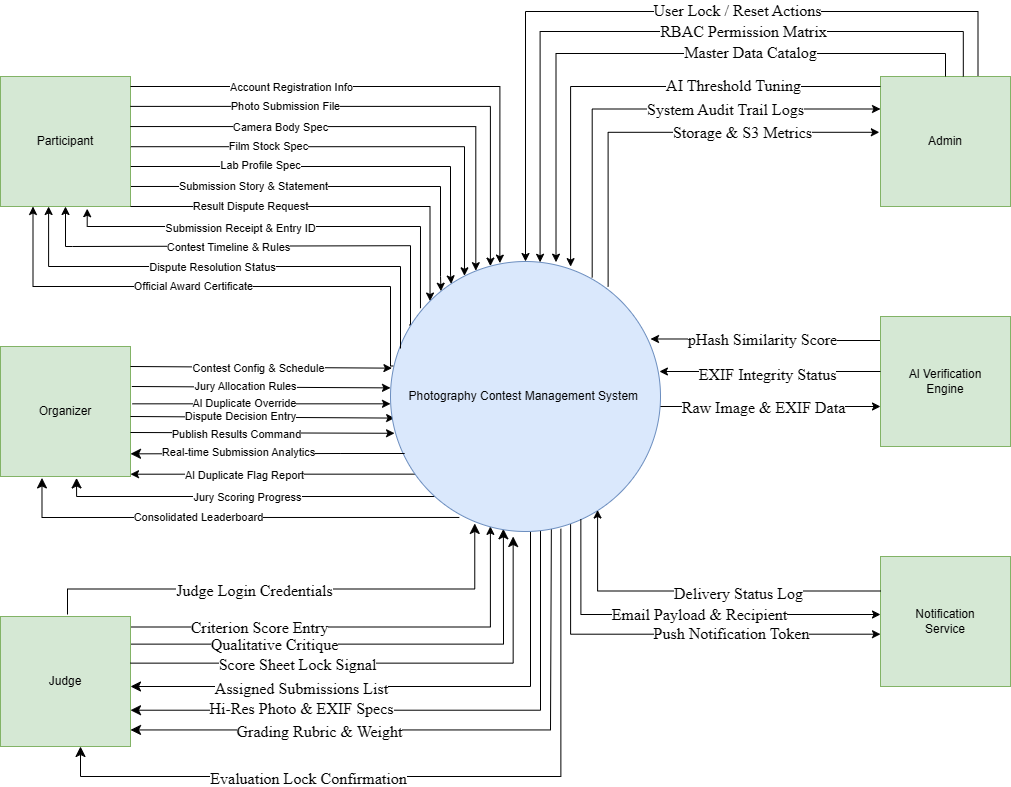
\includegraphics[width=0.95\textwidth]{images/context_diagram}
    \label{fig:context-diagram}
\end{figure}

\subsection{User Requirements}
\label{subsec:user-requirements}

\setcounter{secnumdepth}{4}
\setcounter{tocdepth}{4}
\renewcommand{\theparagraph}{\thesubsubsection.\arabic{paragraph}}

\subsubsection{System Actors}
\label{subsubsec:system-actors}

\renewcommand{\arraystretch}{1.15}
\setlength{\tabcolsep}{6pt}
\begin{longtable}{|>{\centering\arraybackslash}p{0.06\textwidth}|>{\raggedright\arraybackslash}p{0.28\textwidth}|>{\raggedright\arraybackslash}p{0.60\textwidth}|}
\hline
\multicolumn{1}{|c|}{\textbf{No.}} & \multicolumn{1}{c|}{\textbf{Actor}} & \multicolumn{1}{c|}{\textbf{Description}} \\
\hline
\endfirsthead
\multicolumn{1}{|c|}{\textbf{No.}} & \multicolumn{1}{c|}{\textbf{Actor}} & \multicolumn{1}{c|}{\textbf{Description}} \\
\hline
\endhead
\hline
\endfoot
\hline
\endlastfoot
1 & Administrator & Responsible for overall system configuration, managing user accounts, enforcing RBAC (Role-Based Access Control) permissions, tuning AI detection thresholds, managing camera/film master data catalogs, and monitoring system audit trail logs. \\
\hline
2 & Organizer & A contest management authority responsible for setting up competitions, configuring evaluation rubrics, allocating judges, reviewing AI duplicate/fraud flags, handling dispute entries, and publishing final competition results. \\
\hline
3 & Judge & A designated evaluator responsible for logging in, viewing assigned submission queues, evaluating submissions against multi-criteria rubrics, providing qualitative feedback, and locking score sheets. \\
\hline
4 & Participant & A registered user (candidate) who uses the system to browse contests, submit photo entries along with camera/film metadata, track submission status, receive evaluation feedback, and submit result dispute requests. \\
\hline
5 & AI Verification Engine (System Actor) & An external automated service that processes uploaded raw images and EXIF data to compute pHash similarity scores, detect potential duplicate submissions, and flag AI-generated or manipulated images. \\
\hline
6 & Notification Service (System Actor) & An external communication provider responsible for delivering transaction emails, submission receipts, evaluation status updates, and system push notifications to participants and staff. \\
\hline
\end{longtable}

\subsubsection{Use Cases}
\label{subsubsec:use-cases}

\paragraph*{2.2.1 Use Case Diagram}
\label{par:use-case-diagram}
\addcontentsline{toc}{paragraph}{\protect\numberline{2.2.1}Use Case Diagram}

\begin{figure}[htbp]
    \centering
    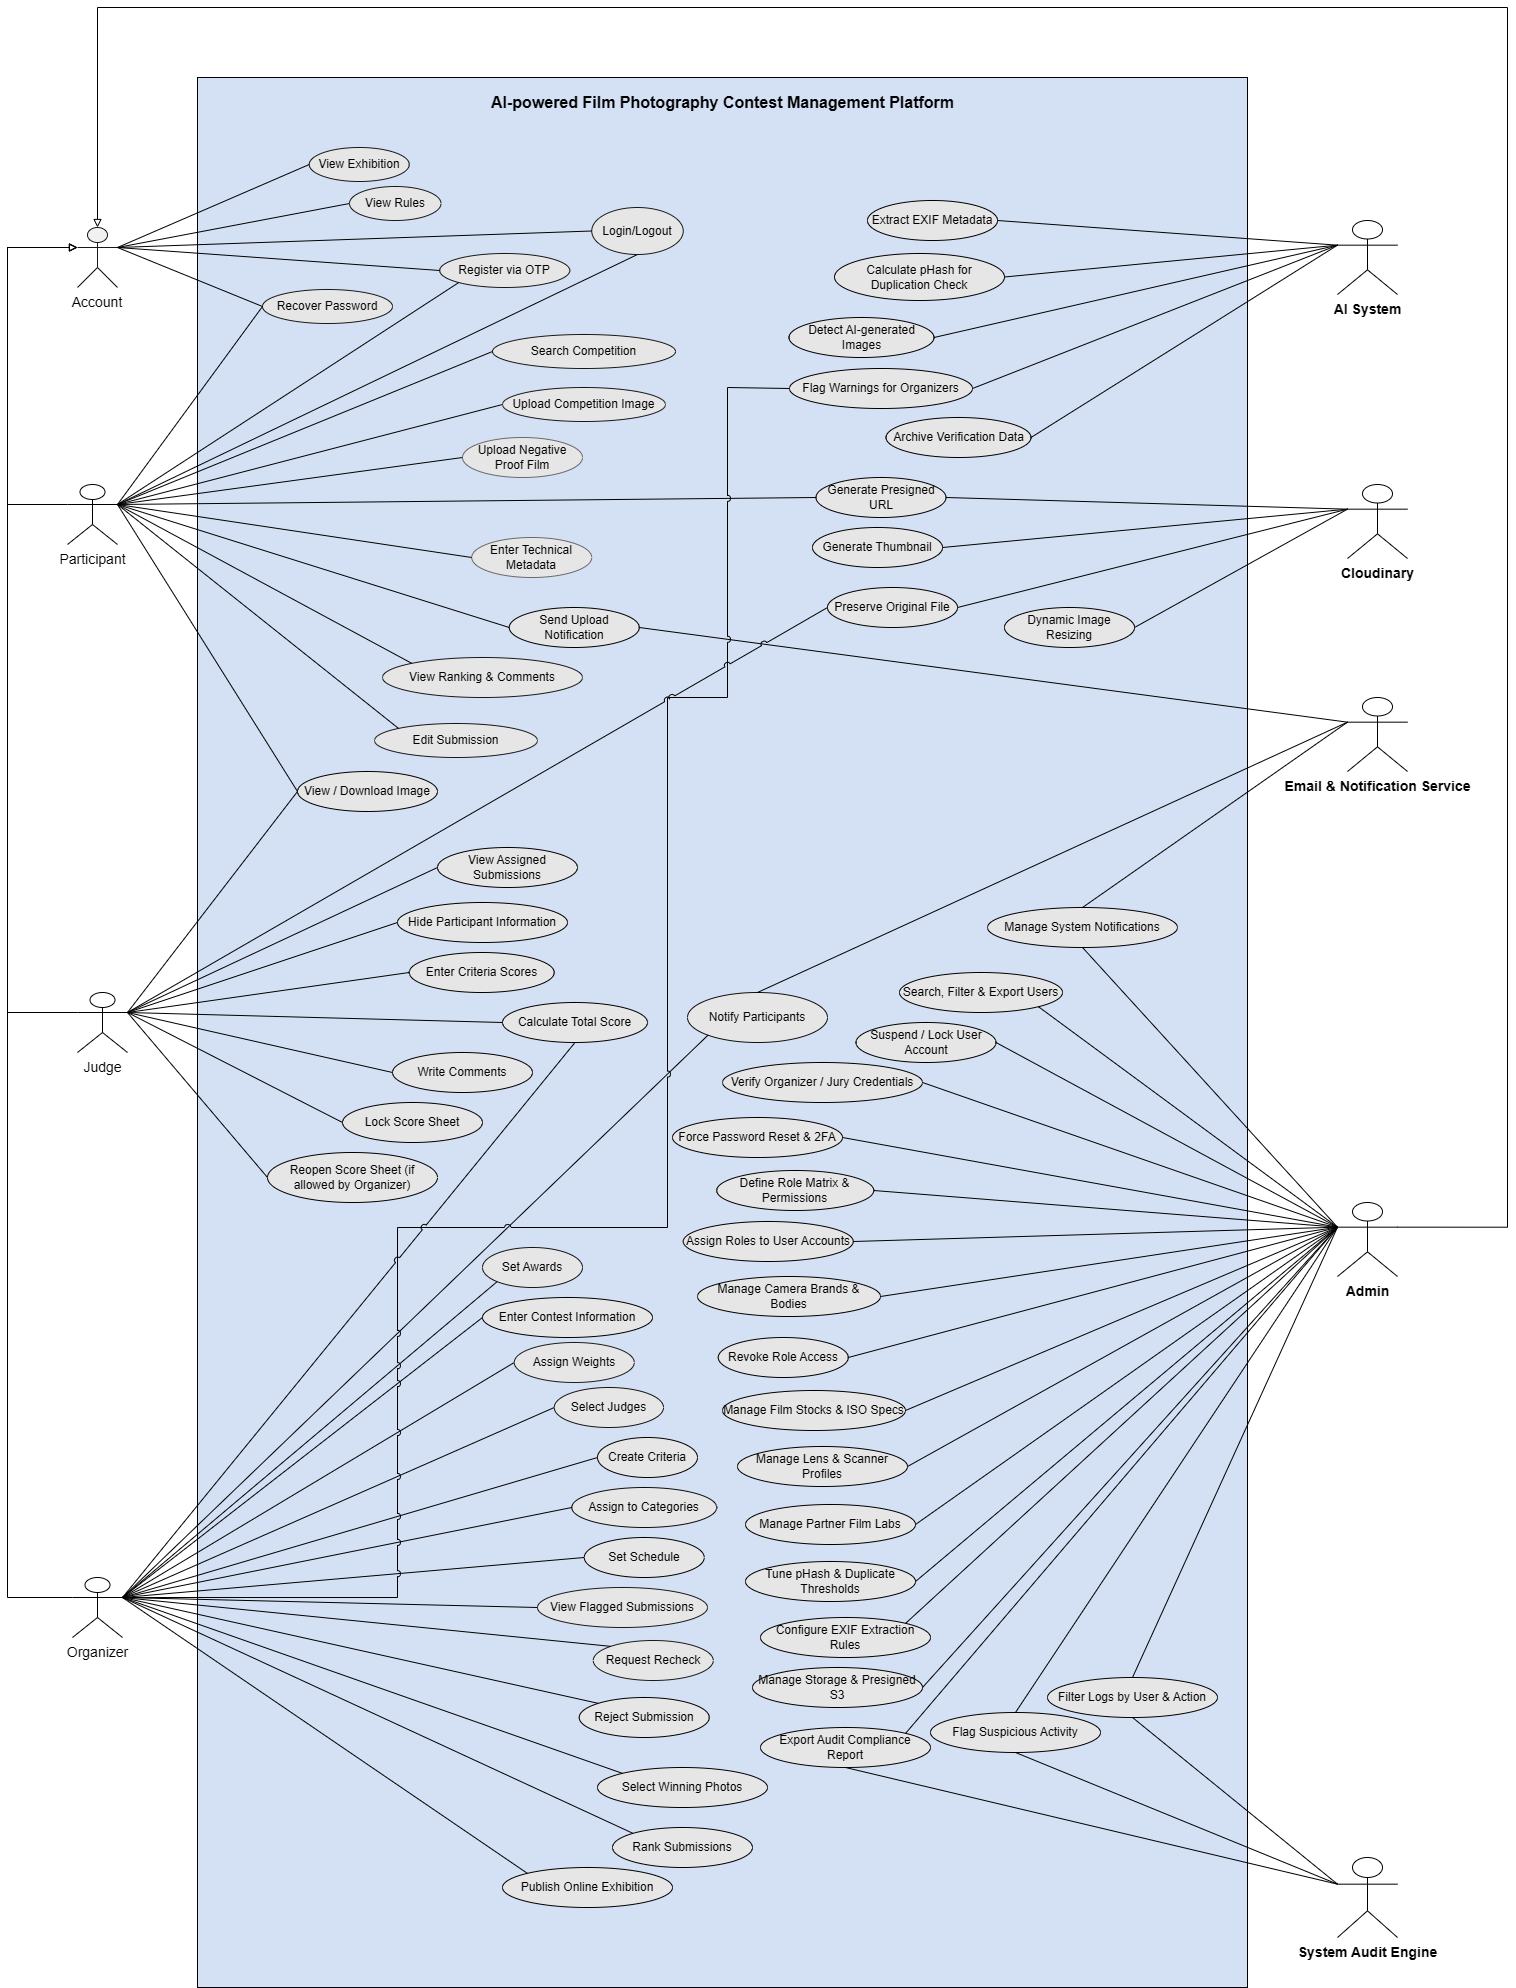
\includegraphics[width=0.95\textwidth]{images/use_case_diagram}
    \label{fig:use-case-diagram}
\end{figure}

\vspace{1em}
\paragraph*{2.2.2 Use Case Descriptions}
\label{par:use-case-descriptions}
\addcontentsline{toc}{paragraph}{\protect\numberline{2.2.2}Use Case Descriptions}

\vspace{0.5em}
\renewcommand{\arraystretch}{1.15}
\setlength{\tabcolsep}{4pt}
\small
\begin{longtable}{|>{\centering\arraybackslash}p{0.07\textwidth}|>{\raggedright\arraybackslash}p{0.20\textwidth}|>{\raggedright\arraybackslash}p{0.20\textwidth}|>{\raggedright\arraybackslash}p{0.45\textwidth}|}
\hline
\multicolumn{1}{|c|}{\textbf{ID}} & \multicolumn{1}{c|}{\textbf{Use Case}} & \multicolumn{1}{c|}{\textbf{Actors}} & \multicolumn{1}{c|}{\textbf{Use Case Description}} \\
\hline
UC-01 & View Exhibition & Account & Allows users to view the exhibition gallery displaying award-winning photo entries from past contests. \\
\hline
UC-02 & View Rules & Account & Displays the rules and regulations of a specific photography contest for users to review before participating. \\
\hline
UC-03 & Login/Logout & Account, Participant & Authenticates users via account credentials to grant access to the system, and allows secure session termination via Logout. \\
\hline
UC-04 & Register via OTP & Account, Participant & Allows users to register a new account using OTP (One-Time Password) verification sent to their email. \\
\hline
UC-05 & Recover Password & Account, Participant & Allows users to reset their forgotten password through email verification. \\
\hline
UC-06 & Search Competition & Participant & Allows participants to search and filter photography competitions by name, category, or status. \\
\hline
UC-07 & Upload Competition Images & Participant & Allows participants to upload their photo entries for a specific competition. \\
\hline
UC-08 & Upload Negative Proof Film & Participant & Allows participants to upload negative proof film images as evidence to verify the authenticity of their photo entries. \\
\hline
UC-09 & Enter Technical Metadata & Participant & Allows participants to input technical metadata for their submitted photo, such as camera, lens, ISO, aperture, and shutter speed. \\
\hline
UC-10 & Send Upload Notification & Participant, Email \& Notification Service & Automatically sends a notification to the participant's email confirming that their upload has been received. \\
\hline
UC-11 & Generate Presigned URL & Participant, Cloudinary & Generates a secure, time-limited URL that allows the participant's browser to upload images directly to Cloudinary storage. \\
\hline
UC-12 & View Ranking \& Comments & Participant & Allows participants to view their ranking results and comments left by judges for their submitted entries. \\
\hline
UC-13 & Edit Submission & Participant & Allows participants to edit the details of a previously submitted entry before the submission deadline. \\
\hline
UC-14 & View/Download Image & Participant, Judge & Allows participants and judges to view or download submitted images in their original quality for review or reference. \\
\hline
UC-15 & Preserve Original File & Judge, Cloudinary & Ensures that the original uploaded image is securely stored in Cloudinary without modification, allowing judges to access the original file whenever needed. \\
\hline
UC-16 & View Assigned Submissions & Judge & Allows the Judge to view the list of submissions assigned to them by the Organizer for a given contest category or judging round, including entry thumbnail, ID, and technical metadata, before starting evaluation. \\
\hline
UC-17 & Hide Participant Information & Judge & Enables blind (anonymous) judging by hiding the submitting participant's identifying information (name, account, portfolio link) from the Judge's view during scoring, ensuring an unbiased evaluation. \\
\hline
UC-18 & Enter Criteria Scores & Judge & Allows the Judge to input a numerical score for each submission against every evaluation criterion (e.g., creativity, composition, technical execution, film grain) defined by the Organizer for that contest. \\
\hline
UC-19 & Calculate Total Score & Judge, Organizer & Automatically computes the weighted total score for each submission by combining the individual criterion scores entered by the Judge with the weight assigned to each criterion, used by the Organizer to determine rankings. \\
\hline
UC-20 & Write Comments & Judge & Allows the Judge to add a qualitative critique or feedback text for a submission alongside its numeric score, providing context for the participant and the Organizer. \\
\hline
UC-21 & Lock Score Sheet & Judge & Allows the Judge to lock their score sheet for a submission once evaluation is complete, preventing further edits and confirming the score as final. \\
\hline
UC-22 & Reopen Score Sheet & Judge, Organizer & Allows the Organizer to unlock a previously locked score sheet (e.g., on the Judge's request or in case of an error/dispute), enabling the Judge to revise scores or comments before results are finalized. \\
\hline
UC-23 & Flag Warmings for Organizers & Organizer, AI System & The AI System automatically flags a submission with a warning — such as a duplicate (pHash) match, suspected AI-generated content, or EXIF inconsistency — and sends the flag report to the Organizer for manual review. \\
\hline
UC-24 & Notify Participants & Organizer, Email \& Notification Service & Allows the Organizer to trigger notifications (email/push) to participants regarding contest updates, submission status, dispute outcomes, or final results, delivered through the Notification Service. \\
\hline
UC-25 & Set Awards & Organizer & Allows the Organizer to define the award structure for a contest, including award categories, number of winners per category, and prize details. \\
\hline
UC-26 & Enter Contest Information & Organizer & Allows the Organizer to create and configure a new contest by entering its name, theme, categories, timeline, and rules. \\
\hline
UC-27 & Assign Weights & Organizer & Allows the Organizer to configure the weight (percentage contribution) of each judging criterion used when calculating a submission's total score. \\
\hline
UC-28 & Select Judges & Organizer & Allows the Organizer to select and assign Judges to a contest or specific category, including allocating them to particular judging rounds. \\
\hline
UC-29 & Create Criteria & Organizer & Allows the Organizer to define and manage the set of scoring criteria (e.g., creativity, storytelling, technical execution) that Judges will use to evaluate submissions in a contest. \\
\hline
UC-30 & Assign to Categories & Organizer & Allows the Organizer to classify and assign submitted photographs to their appropriate contest categories or divisions for organized judging and ranking. \\
\hline
UC-31 & Set Schedule & Organizer & Allows the Organizer to configure the contest timeline, including submission period, judging period, recheck deadline, and winner announcement schedule. \\
\hline
UC-32 & View Fagged Submissions & Organizer & Displays the list of submissions flagged by the AI verification system for duplicate detection, AI-generated content, or metadata inconsistencies, allowing the Organizer to review them. \\
\hline
UC-33 & Request Recheck & Organizer & Enables the Organizer to request an additional review for a submission when suspicious content or scoring discrepancies are identified. \\
\hline
UC-34 & Reject Submission & Organizer & Allows the Organizer to reject submissions that violate contest regulations, fail verification, or do not meet eligibility requirements. \\
\hline
UC-35 & Select Winning Photos & Organizer & Enables the Organizer to select winning submissions based on judges' scores, contest rules, and verification results before publication. \\
\hline
UC-36 & Rank Submissions & Organizer & Automatically or manually ranks submissions according to judges' scores and predefined contest criteria to determine final standings. \\
\hline
UC-37 & Publish Online Exhibition & Organizer & Allows the Organizer to publish approved winning photos to the online exhibition, making them available for public viewing. \\
\hline
UC-38 & Extract EXIF Metadata & AI System & Automatically extracts EXIF metadata from uploaded images to verify camera information, capture settings, and image authenticity. \\
\hline
UC-39 & Calculate pHash for Duplication Check & AI System & Generates perceptual hash (pHash) values to compare uploaded images and identify duplicate or highly similar submissions. \\
\hline
UC-40 & Detect AI-generated Images & AI System & Analyzes uploaded images using AI detection techniques to identify whether the image was generated or manipulated by artificial intelligence. \\
\hline
UC-41 & Archive Vertification Data & AI System & Stores verification results, extracted metadata, and AI analysis records for auditing, dispute resolution, and future reference. \\
\hline
UC-42 & Generate Thumbnail & Cloudinary & Automatically generates optimized thumbnail versions of uploaded images for previews, galleries, and faster loading. \\
\hline
UC-43 & Dynamic Image Resizing & Cloudinary & Dynamically resizes images into different resolutions while preserving image quality for various display devices. \\
\hline
UC-44 & Manage System Notifications & Admin, Email \& Notification Service & Allows the Admin to configure notification templates and events, while the Email Notification Service delivers OTPs, status updates, and contest notifications to users. \\
\hline
UC-45 & Search, Filter \& Export Users & Admin & Enables the Admin to search, filter, and export user information for administration, reporting, and system management purposes. \\
\hline
UC-46 & Suspend/Lock User Account & Admin & Allows the Admin to temporarily suspend or permanently lock user accounts upon detecting policy violations. \\
\hline
UC-47 & Verify Organizer/Jury Credentials & Admin & Allows the Admin to verify profiles and approve the identities and credentials of Organizers or Jury members. \\
\hline
UC-48 & Force Password Reset \& 2FA & Admin & Allows the Admin to force users to reset their passwords and set up Two-Factor Authentication (2FA) upon their next login. \\
\hline
UC-49 & Define Role Matrix \& Permissions & Admin & Allows the Admin to configure the role-based access control (RBAC) matrix, specifying detailed permissions for each system role. \\
\hline
UC-50 & Assign Roles to User Accounts & Admin & Allows the Admin to assign specific roles and privileges to individual user accounts within the system. \\
\hline
UC-51 & Manage Camera Brands \& Bodies & Admin & Allows the Admin to add, update, or delete categories of analog camera brands and camera bodies. \\
\hline
UC-52 & Revoke Role Access & Admin & Allows the Admin to partially or fully revoke access permissions previously granted to a user account. \\
\hline
UC-53 & Manage Film Stocks \& ISO Specs & Admin & Allows the Admin to manage the catalog of film stocks and their corresponding ISO specifications. \\
\hline
UC-54 & Manage Lens \& Scanner Profiles & Admin & Allows the Admin to manage configurations and metadata profiles for various camera lenses and film scanners. \\
\hline
UC-55 & Manage Partner Film Labs & Admin & Allows the Admin to add, update, or remove information regarding partner film processing labs. \\
\hline
UC-56 & Tune pHash \& Duplicate Thresholds & Admin & Allows the Admin to adjust the pHash algorithm and similarity thresholds to optimize the detection of duplicate or plagiarized images. \\
\hline
UC-57 & Configure EXIF Extraction Rules & Admin & Allows the Admin to define rules for parsing and extracting EXIF metadata from uploaded images. \\
\hline
UC-58 & Manage Storage \& Presigned S3 & Admin & Allows the Admin to manage storage capacity and configure secure upload links (Presigned URLs) via Amazon S3. \\
\hline
UC-59 & Export Audit Compliance Report & Admin, System Audit Engine & Allows the generation and exporting of audit reports regarding system security compliance and data integrity. \\
\hline
UC-60 & Flag Suspicious Activity & Admin, System Audit Engine & The system automatically flags suspicious activities (e.g., spam, hacking attempts) and alerts the Admin for resolution. \\
\hline
UC-61 & Filter Logs by User & Admin, System Audit Engine & Allows the Admin to search, filter, and view detailed system activity logs for specific user accounts. \\
\hline
\end{longtable}

\end{document}